\documentclass[11pt,english]{article}

%{{{ packages

\usepackage{a4my}
\usepackage[latin1]{inputenc}
\usepackage{babel}

\usepackage{amsmath}
\usepackage{amssymb}
\usepackage{theorem}
\usepackage{latexsym}

\usepackage{ifthen}
\usepackage{xspace}

\usepackage{epsfig}
\usepackage[hang]{subfigure}
\usepackage{float}
\setcounter{topnumber}{3}

\usepackage{hangftn}
\usepackage{hangcap}
\usepackage[square,authoryear]{natbib}
\usepackage{fancyheadings}

%}}}

%{{{ definitions :

\newcommand{\xc}{x_{cur}}
\newcommand{\xg}{x_{goal}}
\newcommand{\xs}{x_{stop}}
\newcommand{\ts}{t_{stop}}
\newcommand{\vc}{v_{cur}}
\newcommand{\vm}{v_{max}}
\newcommand{\am}{a_{max}}
\newcommand{\half}{\frac{1}{2}}
\newcommand{\abs}[1]{|#1|}
\newcommand{\sgn}{\operatorname{sgn}}

%}}}

\begin{document}
\title{Smooth Trajectory Planner (STP)}
\author{Robert Haschke}
\maketitle

\section{Fastest trajectory}
Planning a smooth trajectory between some current position $\xc$ and a target
position $\xg$ means to connect these points by a smooth, i.e. continously
differentiable curve. This can be achieved easiest by concatenating
\begin{itemize}\itemsep0pt
\item an acceleration phase (linearly increasing speed): 
  $a(t) = a_0 + a_1 t + a_2 t^2$
\item a cruising phase (constant speed): $c(t) = c_0 + c_1 t$
\item a deceleration phase (linearly decreasing speed):
  $d(t) = d_0 + d_1 t + d_2 t^2$
\end{itemize}
If we denote the switching time between acceleration and cruise by $t_1$, the
switching time between cruise and deceleration by $t_2$ and the duration of
the movement by $t_3$ the whole movement can be composed as follows (see
fig.~\ref{fig:simple}):
\begin{equation*}
  x(t) = \begin{cases}
    a(t) \quad t < t_1 \\
    c(t) \quad t < t_2 \\
    d(t) \quad t < t_3 \\
    \xg  \quad \text{else}
  \end{cases}
\end{equation*}
\begin{figure}
  \begin{minipage}[t]{0.45\linewidth}
    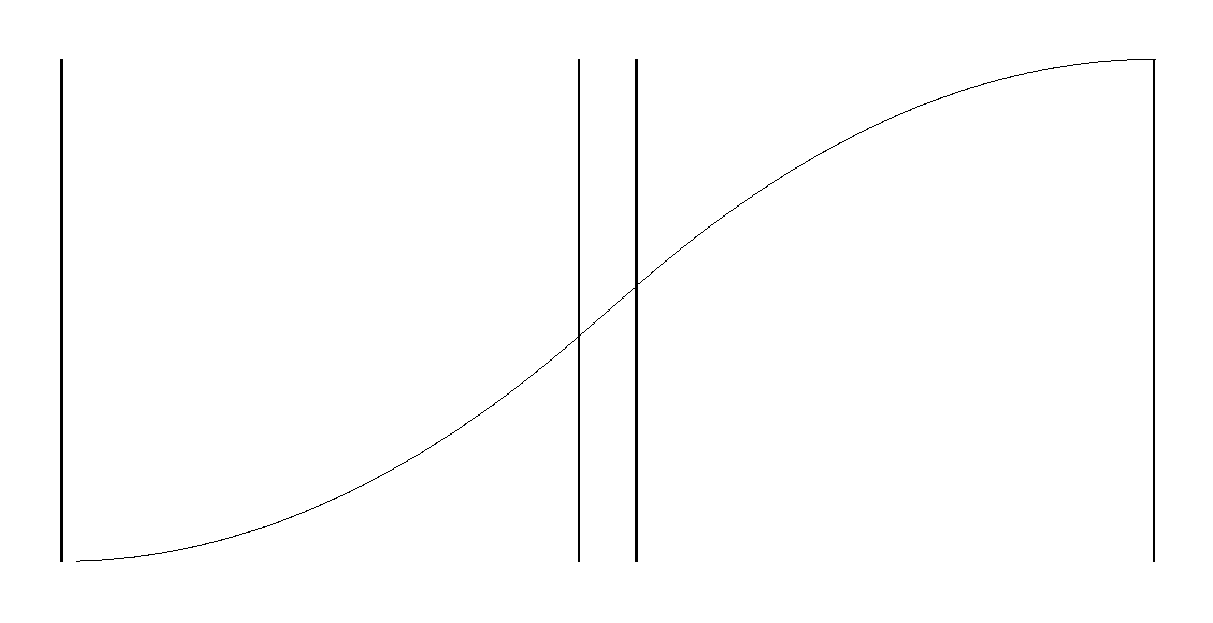
\includegraphics[width=\linewidth]{simple-x.eps}
    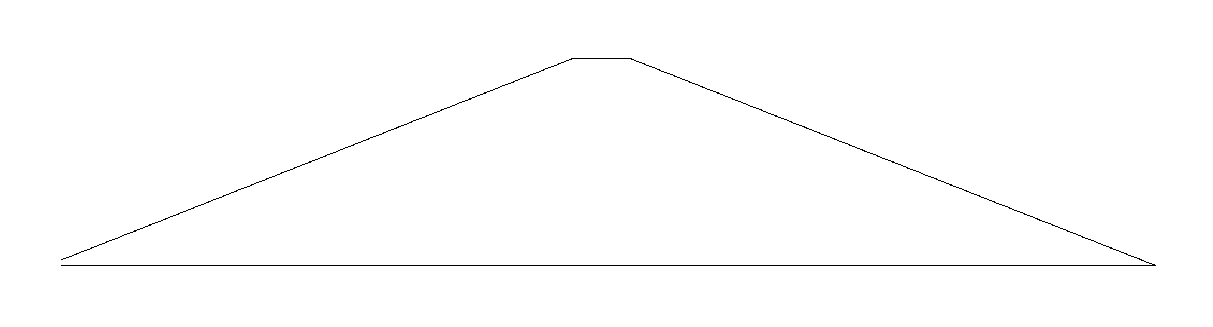
\includegraphics[width=\linewidth]{simple-v.eps}
    \caption{Smooth trajectory composed of acceleration, cruising and
      deceleration phase. Velocity shows a trapezoidal profile.}
    \label{fig:simple}
  \end{minipage}\hfill
  \begin{minipage}[t]{0.45\linewidth}
    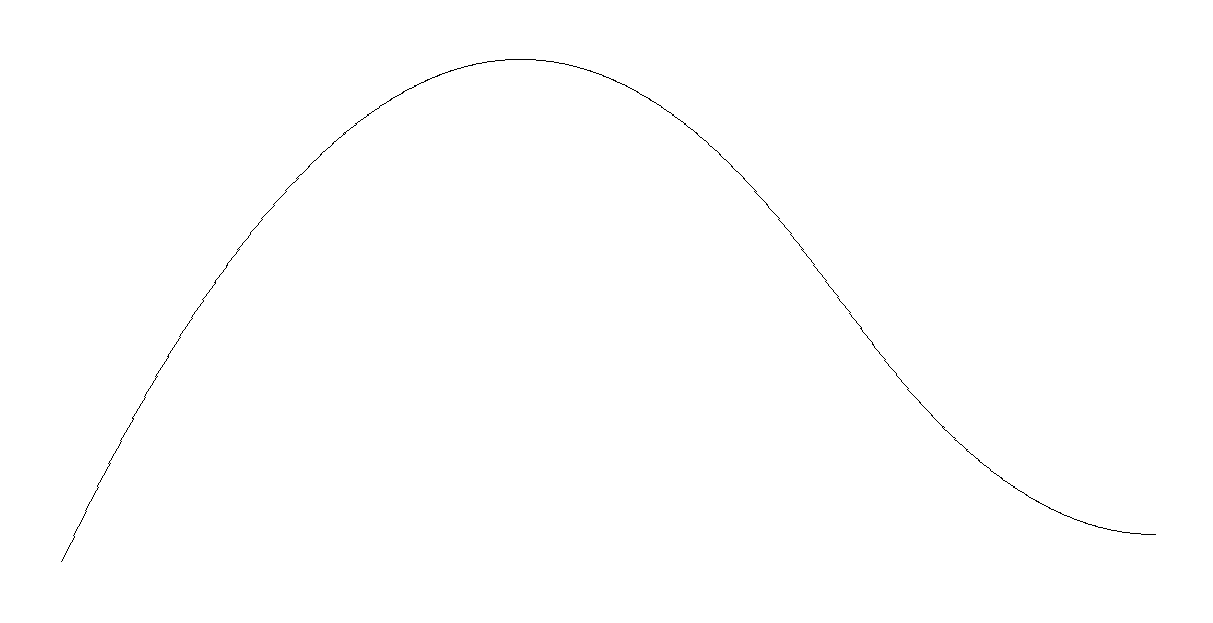
\includegraphics[width=\linewidth]{overshoot-x.eps}
    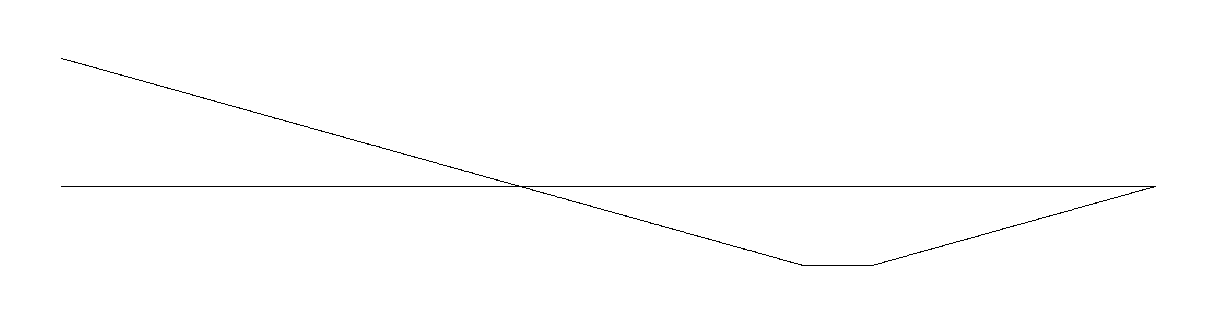
\includegraphics[width=\linewidth]{overshoot-v.eps}
    \caption{If full stop overshoots new target, the direction of cruising
      phase switches sign!}
    \label{fig:overshoot}
  \end{minipage}
\end{figure}
The magnitude of acceleration or deceleration is fixed to $\am$. Hence $|a_2|
= |d_3| = \half \am$. The first task to solve, is to decide for the direction
$d \in \{-1,1\}$ of cruising, which automatically determines the (default)
direction of acceleration and deceleration phase:
\begin{alignat*}{2} 
  a_2 &= \phantom{-}\half d \am = \half acc &\qquad acc &:= \phantom{-}d \am \\
  d_2 &= -\half d \am = \half dec &\qquad dec &:= -d \am
\end{alignat*}

At first glance this is easy, simply choose $d=\sgn(\xg - \xc)$. But, the
problem is, that we want to be able to smoothly switch to another target at
arbitrary time (preferably after cruising phase). Hence we must be able to
cope with some initial speed $\vc$. If this speed is too large, such that we
even overshoot the new target $\xg$, if we would immediately stop with
maximally available deceleration, the direction $d$ actually changes (see fig.~\ref{fig:overshoot})!
Hence, first we have to compute the final position $\xs$ after an immediate
stop: 
\begin{align*}
  \text{time needed to stop:}& \qquad&
  \ts &= \frac{\abs{\vc}}{\am} \\
  \text{final position after stop:}& \qquad&
  \xs &= \xc + \ts \cdot (\vc - \sgn(\vc) \cdot \half \am \cdot \ts)
\end{align*}
Now we can compute the direction of cruising phase: $d = \sgn (\xg - \xs)$.

Next we have to compute the duration of cruising phase. For this purpose we
first assume it is nonzero. Hence we compute the time $\Delta t_1$ needed to
reach cruising speed $c_1 = d \vm$ and time $\Delta t_2$ to stop from cruising
speed together with the respective changes of position $\Delta x_1$ and
$\Delta x_2$:
\begin{alignat*}{2}
  \Delta t_1 &= \frac{d \, \vm - \vc}{acc} &\qquad
  \Delta x_1 &= \Delta t_1 \cdot (\vc + \half acc \cdot \Delta t_1) \\
  \Delta t_2 &= \frac{\vm}{\am} &\qquad
  \Delta x_2 &= \Delta t_2 \cdot (d \, \vm + \half dec \cdot \Delta t_2)
\end{alignat*}
The time $\Delta t_1$ may become negative, if the current velocity $|\vc|$ is
larger in magnitude than the new maximum velocity $\vm$. In this case, obviously the velocity has to be decreased with maximum deceleration and the direction of the acceleration phase switches its sign. Hence we change these values:
\begin{align*}
  acc' &= -acc \\
  \Delta t'_1 &= - \Delta t_1
\end{align*}
Now the cruising duration can be easily computed:
\begin{align*}
  T_c = \frac{\xg - (\xc + \Delta x_1 + \Delta x_2)}{d \, \vm}
\end{align*}
If this duration is indeed positive, we can plan a full trapezoidal velocity
profile:
\begin{alignat*}{2}
  &\text{Duration:} &\qquad t_3 &= \Delta t_1 + T_c + \Delta t_2 \\
  &\text{acceleration phase:} &\qquad t_1 &= \Delta t_1\\
  &\text{deceleration phase:} &\qquad t_2 &= t_3 - \Delta t_2\\
  &\text{cruising speed:} &\qquad c_1 &= d \, \vm
\end{alignat*}
If its negative, the position change within acceleration and deceleration
phase ($\Delta x_1 + \Delta x_2$) already overshoots the target and we must
omit the cruising phase and simultaneously shorten the acceleration and
deceleration phases. Hence we neither know the duration times $\Delta t_1$,
$\Delta t_2$ of acceleration and deceleration phase nor the magnitude $w =
\abs{c_1}$ of cruising speed. But they satisfy the following equations:
\begin{alignat*}{2}
  \Delta t_1 &= \frac{d \, w - \vc}{d \, \am} \qquad&
  \Delta x_1 &= \Delta t_1 \cdot (\vc + \half d \, \am \cdot \Delta t_1) \\
  \Delta t_2 &= \frac{w}{\am} \qquad&
  \Delta x_2 &= \Delta t_2 \cdot (d \, w - \half d \, \am \cdot \Delta t_2) \\
  &\qquad \xg - \xc &=\quad \Delta x_1 + \Delta x_2
\end{alignat*}
In this case, $\Delta t_1$ cannot become negative, although its expression has
a similar form as before. The reason is the following: The incomplete,
triangular velocity profile branch is only entered if the position change from
first and third phase (which will be decelerations both if $\Delta t_1$ became
negative before) would already overshoot the desired target. But, overshooting
the target by a full stop is already handled at the very beginning and
requires a deceleration followed by an acceleration back to the target.

Solving the above equations for $w$ yields:
\begin{alignat*}{2}
  &\text{magnitude of cruising speed:} &\qquad 
  w &= \sqrt{d \, \am \, (\xg - \xc) + \half \vc^2} \\
  &\text{cruising speed:} &\qquad c_1 &= d \, w \\
  &\text{acceleration phase:} &\qquad 
  t_1 &= t_2 = \Delta t_1 = \frac{d \, w - \vc}{d \, \am}\\
  &\text{Duration:} &\qquad t_3 &= \Delta t_1 + \Delta t_2
\end{alignat*}
All remaining parameters can be easily computed:
\begin{alignat*}{3}
  a_2 &= \half \, acc&\qquad
      &{}&\qquad
  d_2 &= \half \, dec \\
%
  a_1 &= \vc &\qquad
  c_1 &{}&\qquad
  d_1 &= c_1 - 2 \, d_2 \, t_2 \\
%
  a_0 &= \xc &\qquad
  c_0 &= a_0 + t_1 \, (a_1 + a_2 \, t_1) - c_1 \, t_1 &\qquad
  d_0 &= c_0 + t_2 \, c_1 - t_2 \, (d_1 + d_2 \, t_2) \\
  &{}&{}&{}&{}&= c_0 + d_2 \, t_2^2
\end{alignat*}

\section{Synchronous Evolution of multiple DOFs}
Commonly we have to control several DOFs and we typically want that all DOFs
finish their movements simultaneously. This requires to scale the whole
trajectory to a new duration $T$, i.e. the duration of the slowest joint. Such
an ability to scale is also necessary due to the need for a finite sampling
time $\Delta t$. If the movement has to be finished after $N$ time steps of
length $\Delta t$, the trajectory has to be scaled to a duration of $N \cdot
\Delta t$. The number of necessary steps can be easily computed:
\begin{equation*}
  N = \left\lfloor \frac{t_3}{\Delta t} \right\rfloor + 1
\end{equation*}

\subsection{Achieving straight lines in configuration space}
If straight lines in configuration space are desired, all DOFs even have to
evolve synchronously, especially they must have identically shaped velocity
profiles and identical lengths of acceleration, cruising and deceleration
phases. This results from the fact, that a straight line is achieved with a
common time evolution $t \in [0..T] \mapsto \tau(t)\in[0..1]$ for all joints
only:
\begin{gather*}
  \vec{x}(t) = \vec{x}_{cur} + \tau(t) \cdot (\vec{x}_{goal} - \vec{x}_{cur})
  = \vec{x}_{cur} + \tau(t) \cdot \vec{\Delta} \qquad\qquad
  \dot{\vec{x}} = \dot{\tau} \cdot \vec{\Delta} \qquad
  \ddot{\vec{x}} = \ddot{\tau} \cdot \vec{\Delta}
\end{gather*}
Hence, the velocity and acceleration only depends on $\dot\tau$ resp.
$\ddot\tau$ and the desired change $\Delta_i$ of a particular component. Given
nonzero initial velocities, it is unlikely, that their distribution exactly
matches the distribution of changes $\Delta_i$ which would be the only
possibility to represent the situation with the above model relying
on the scalar scaling factor $\dot\tau(0)$ only.

\subsection{Adapt trajectory to given duration}
If curved trajectories in configuration space are allowed, a rescaling is
possible also in the general case of nonzero starting velocities.
The naive approach to do the scaling would be to scale all variables
appropriately using the factor $s = t_3 / T$:
\begin{alignat*}{4}
  a_2 &= a_2 \cdot s^2 &\qquad &&\qquad d_2 &= d_2 \cdot s^2 &\qquad 
  t_3 &= t_3 / s \\
  a_1 &= a_1 \cdot s &\qquad c_1 &= c_1 \cdot s &\qquad d_1 &= d_1 \cdot s 
  &\qquad t_2 &= t_2 / s \\
  && && && t_1 &= t_1 / s
\end{alignat*}
This works well, if the initial speed $\vc$ and hence $a_1$ is zero. In any
other case, $a_1$ is scaled leaving a gap between real speed $\vc$ and new
starting speed $a_1 = s \cdot \vc$ (see fig.~\ref{fig:NaiveScale}). Hence, a
more elaborated approach is needed. The idea of the presented approach is to
shorten both the acceleration and deceleration phase by some amount $\Delta$.
This decreases the magnitude of the cruising speed by $\Delta v = \Delta \cdot
\am$ and the magnitude of position change in acceleration as well as
deceleration phase by $\Delta x = \Delta \cdot (v_c^o - \half a \cdot
\Delta)$, where $v_c^o=\abs{c_1}$ is the old cruising speed. Denoting the old
resp. new duration by $T^o$ and $T^n$ and using the already introduced
notation extended by an upper index $^o$ or $^n$ for old resp. new values, we
can formulate the following equations:
\begin{gather*}
  T^n = \Delta t_1^n + T_c^n + \Delta t_2^n \tag{1}\\
  T^o = \Delta t_1^n + \Delta + T_c^o + \Delta + \Delta t_2^n =
  \Delta t_1^o + T_c^o + \Delta t_2^o \tag{2}\\
  T^n - T_c^n = T^o - T_c^o - 2 \, \Delta \tag{1+2}\\
  \Delta x = \Delta \cdot (v_c^o - \half a \cdot \Delta) \\
  v_c^n = \frac{v_c^o \cdot T_c^o + 2 \, \Delta x}{T_c^n} = v_c^o - a \, \Delta
\end{gather*}
Solving this equation for $\Delta$ leads to:
\begin{align*}
  \Delta &= -\frac{B}{2} + \sqrt{\frac{B^2}{4} + A} \\
  \text{where}\qquad B &= T^n - T^o + T_c^o \\
  A &= (T^n - T^o) \frac{v_c^o}{\am} \geq 0
\end{align*}
and we can easily correct all parameters ($^n$ omitted):
\begin{alignat*}{3}
  t_1 &= t_1^o - \Delta &\qquad 
  c_1 &= a_1 + 2 \, a_2 \, t_1 &\qquad
  d_1 &= c_1 - 2 \, d_2 \, t_2 \\
%
  t_3 &= T^n &\qquad 
  c_0 &= a_0 + t_1 \, (a_1 + a_2 \, t_1) - c_1 \, t_1 &\qquad
  d_0 &= c_0 + t_2 \, c_1 - t_2 \, (d_1 + d_2 \, t_2) \\
%
  t_2 &= T^n - (T^o - t_2^o - \Delta) &\qquad 
  &&&= c_0 + d_2 \, t_2^2
\end{alignat*}
\begin{figure}
  \centering
  \begin{minipage}[t]{0.45\linewidth}
    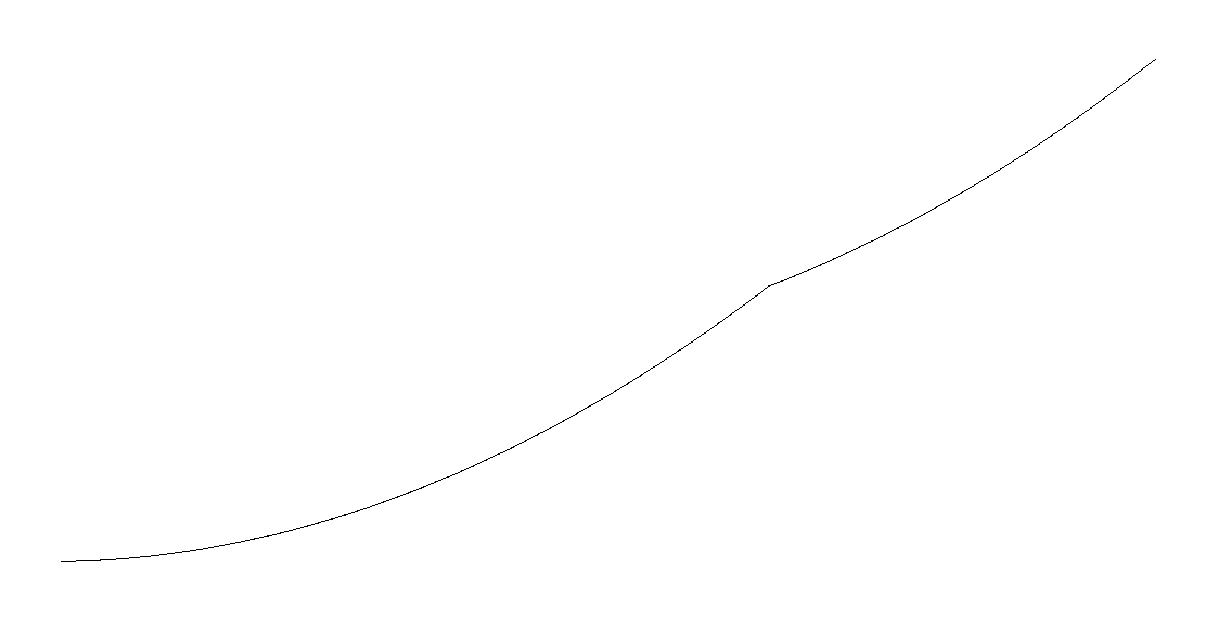
\includegraphics[width=\linewidth]{naivescale-x.eps}
    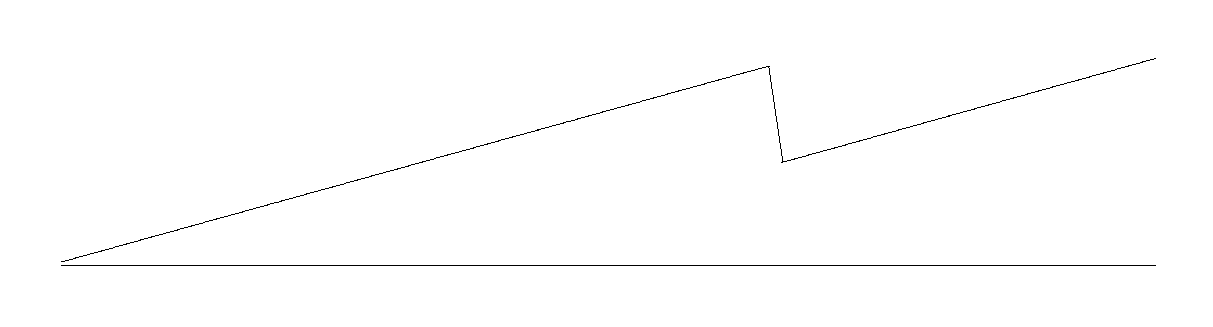
\includegraphics[width=\linewidth]{naivescale-v.eps}
    \caption{Naive scaling to a new duration leads to a gap between current
      speed $\vc$ and new initial speed $a_1 = s \cdot \vc$.}
    \label{fig:NaiveScale}
  \end{minipage}
\end{figure}
Until now we silently assumed that $\Delta t_1^o - \Delta$ is positive leaving
an nonzero acceleration phase. But, if acceleration phase is already very
small (in extreme cases it might be zero, because we can simply go on
cruising), this assumption is not true any longer. Ignoring this case leads to
undesirable behaviour (see fig.~\ref{fig:ScaleErr}). To solve the problem we
have to decelerate in the beginning as well, leaving a smaller magnitude of
cruising speed than before. The time for a full stop is again $\ts = \abs{\vc}
/ \am$. The idea is to cut this deceleration phase and insert a cruising phase
in between to achieve the desired duration (see fig.~\ref{fig:ScaleOK}). This
leads to the following equations:
\begin{gather*}
  T^n = \Delta t_1 + T_c + \Delta t_2 = T_c + \ts \\
  c_1 = \frac{\xg - \xs}{T_c} = \frac{\xg - \xs}{T^n - \ts} \\
  \\
  a_2 = -a_2^o \qquad
  t_1 = \frac{\abs{c_1 - a_1}}{\am} \qquad
  t_2 = T^n - (\ts - t_1) \qquad
  t_3 = T^n
\end{gather*}
\begin{figure}
  \begin{minipage}[t]{0.45\linewidth}
    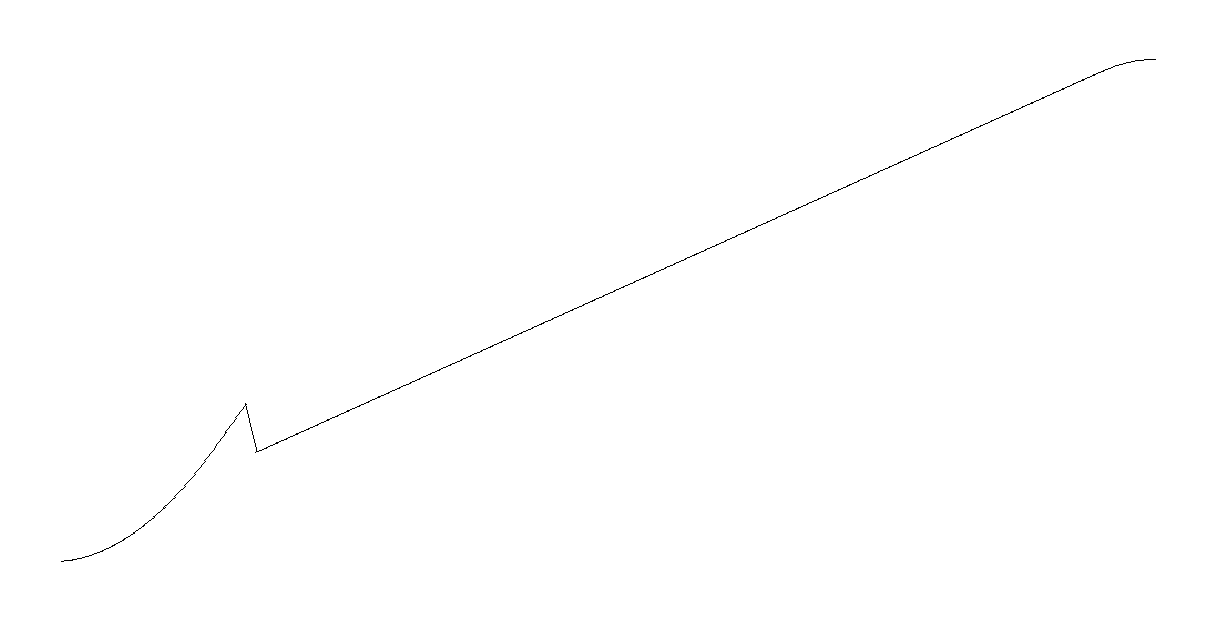
\includegraphics[width=\linewidth]{scaleerr-x.eps}
    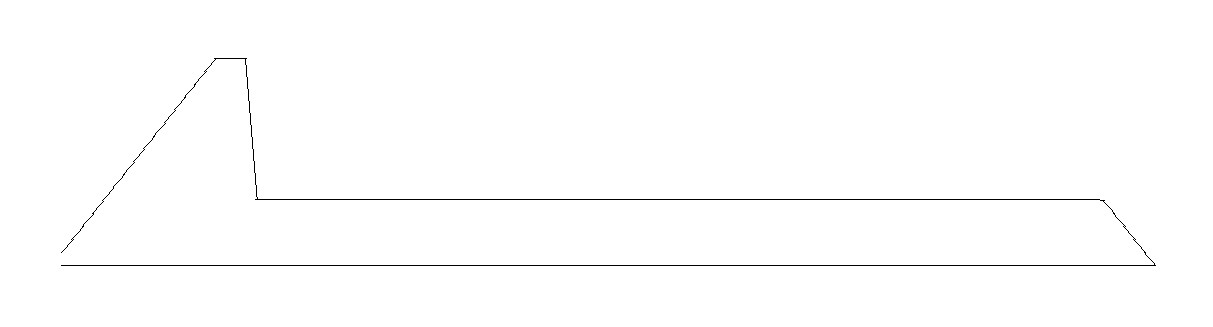
\includegraphics[width=\linewidth]{scaleerr-v.eps}
    \caption{Negative $t_1^n = t_1^o - \Delta$ leads to discontinuous
      trajectories.}
    \label{fig:ScaleErr}
  \end{minipage}\hfill
  \begin{minipage}[t]{0.45\linewidth}
    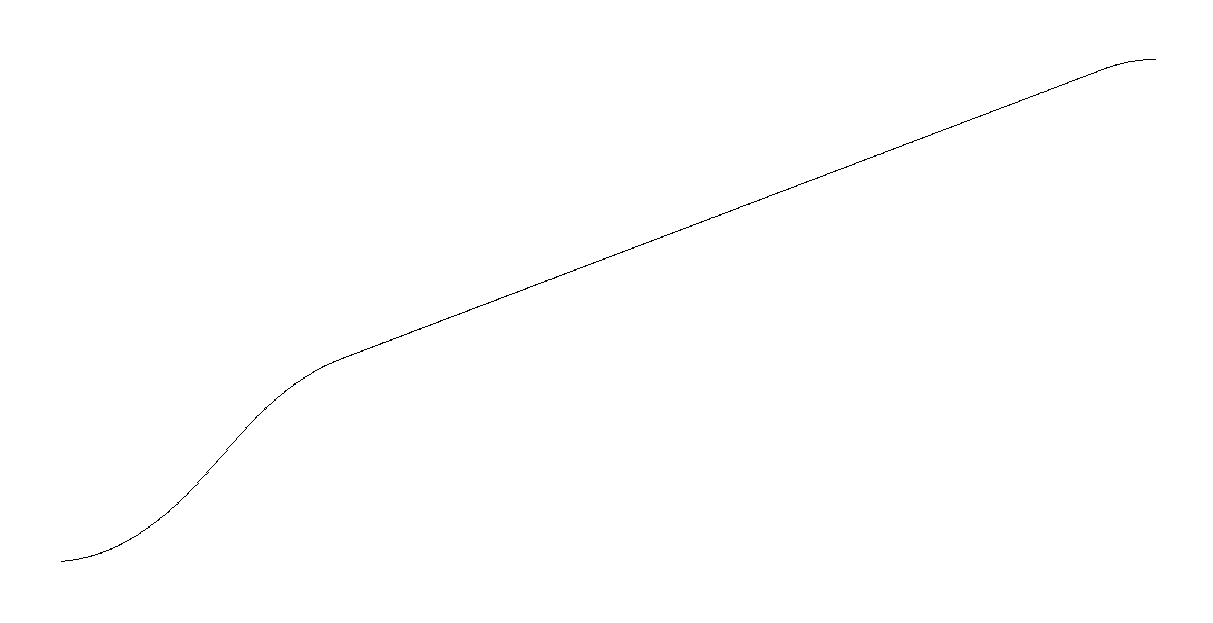
\includegraphics[width=\linewidth]{scaleok-x.eps}
    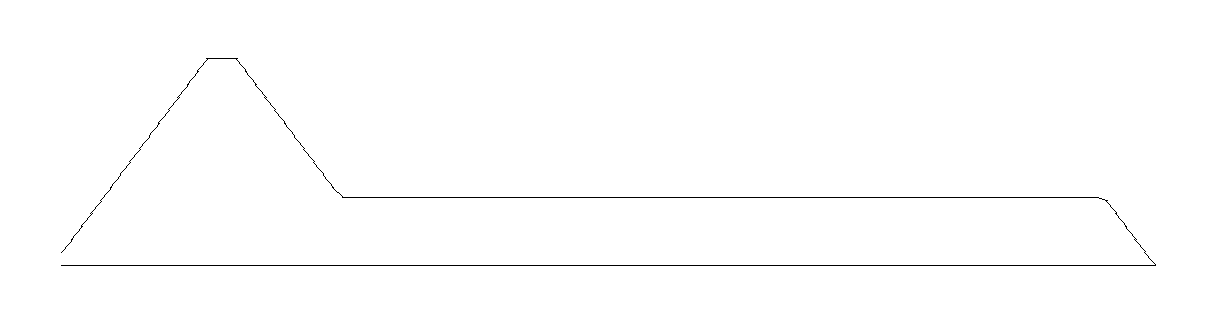
\includegraphics[width=\linewidth]{scaleok-v.eps}
    \caption{The solution is to split the deceleration phase and insert a
      cruising phase of appropriate length.}
    \label{fig:ScaleOK}
  \end{minipage}
\end{figure}

\end{document}
